% Advanced Computer Graphics seminar report
% Topic 2.9: Image-Based Lighting

\newif\ifegtemplate
\IfFileExists{egpubl.cls}{
  \egtemplatetrue
  \documentclass{egpubl}
  \JournalPaper
  \electronicVersion
}{
  \egtemplatefalse
  \documentclass[10pt,twocolumn]{article}
}

\usepackage{graphicx}
\pdfcompresslevel=9
\ifegtemplate
  \PrintedOrElectronic
  \usepackage{t1enc,dfadobe}
  \usepackage{egweblnk}
\else
  \usepackage[T1]{fontenc}
  \usepackage[margin=1.8cm]{geometry}
  \usepackage{times}
  \usepackage{url}
\fi
\usepackage{cite}
\usepackage{booktabs}
\usepackage{amsmath}
\newcommand{\code}[1]{{\scriptsize\texttt{#1}}}

\title{Image-Based Lighting}

\author{Dino Džaferagić\\
University of Ljubljana, Faculty of Computer and Information Science\\
\texttt{dd5102@student.uni-lj.si}}

\begin{document}

\maketitle

\begin{abstract}
    Realistic lighting is hard because light reaches an object from many directions, not only from one lamp.
    This project implements a real-time image-based lighting renderer in WebGPU.
    The renderer loads HDR environment maps, converts them to cubemaps, and builds textures for diffuse and specular lighting.
    It uses diffuse irradiance, a GGX prefiltered environment map, and a BRDF lookup table for the split-sum approximation.
    The final shader renders a procedural sphere and Stanford models with a simple PBR material.
    The results show that changing the environment, metallic value, and roughness changes the final image in a clear way.
    The renderer runs in real time, but it does not replace full global illumination or path tracing.
\end{abstract}

\section{Introduction}

Realistic lighting is difficult in real-time graphics because a surface receives light from the whole scene around it.
A small set of point lights cannot capture this effect well.
Image-based lighting (IBL) uses an HDR image of the environment as a light source.
The image stores incoming light from many directions and can light synthetic objects as if they were placed in that environment.

The goal of this seminar was to build a real-time IBL renderer in WebGPU.
The project supports a procedural sphere, the Stanford Bunny, and the Stanford Dragon.
It also includes UI controls for the environment, material parameters, IBL terms, and performance statistics.
This report describes the implementation and evaluates the visual result and runtime cost.

\section{Background}

Paul Debevec's work on image-based lighting shows how measured light from a real environment can illuminate synthetic objects \cite{debevec2006ibl,debevec1999ibml}.
The main input is an HDR environment map.
HDR is important because light sources and bright sky regions can be much brighter than normal display colors.
The implementation uses Radiance RGBE \texttt{.hdr} files, which store RGB values with a shared exponent.

The downloaded HDR maps use an equirectangular layout.
This layout stores longitude in the horizontal axis and latitude in the vertical axis.
For rendering, the map is converted to a cubemap.
A cubemap is easier to sample with a 3D direction vector.

Diffuse IBL needs the average incoming light over the hemisphere around a surface normal.
The renderer precomputes this into a low-resolution irradiance cubemap.
Specular IBL needs rough reflections.
The renderer precomputes a GGX-filtered cubemap with mip levels, where higher mip levels match higher roughness.
The BRDF integration LUT stores the second part of the split-sum approximation.
At runtime the shader uses material parameters such as albedo, metallic, and roughness to combine these textures.

\section{Method and Implementation}

\subsection{WebGPU Renderer}

The project uses TypeScript, Vite, WebGPU, and WGSL shaders.
The render loop creates WebGPU render passes for the skybox, final PBR object, and comparison views.
The UI is plain HTML and updates the renderer state each frame.
The camera uses a simple orbit controller.

HDR data is stored in \texttt{rgba16float} textures.
This format keeps values in linear HDR space and avoids the need for optional 32-bit float texture filtering.
The renderer applies tone mapping and gamma correction only at the end of the final shader.
This keeps lighting math in linear space.

\subsection{Environment Map Preprocessing}

The preprocessing code is implemented in the IBL module.
The main files are \code{processor.ts} and \code{iblPreprocess.ts}.
It runs when an environment is first selected.
The pipeline has these steps.

First, the loader reads the RGBE \texttt{.hdr} file and decodes it into linear floating-point RGB values.
The data is converted to half-float RGBA and uploaded to WebGPU.

Second, a WGSL shader converts the equirectangular map to a cubemap.
The output cubemap has six faces of size $512 \times 512$.
All later IBL textures are built from this cubemap.

Third, the renderer builds a diffuse irradiance cubemap.
For each output direction, the shader samples the hemisphere around the normal and weights each sample by the cosine term.
The result is low frequency by design, so the texture size is $64 \times 64$ per face.

Fourth, the renderer builds a prefiltered specular cubemap.
The base level is $256 \times 256$ per face and the texture has nine mip levels.
Each mip level uses a different roughness value.
The shader uses a Hammersley sequence and GGX importance sampling with 256 samples per face pass.

Fifth, the renderer builds a $256 \times 256$ BRDF integration LUT.
This texture stores scale and bias terms for the split-sum specular approximation.
The final shader samples it with $N \cdot V$ and roughness.

\subsection{PBR Shading}

The final shader is implemented in \code{renderShaders.ts}.
For each fragment it computes the normal $N$, the view direction $V$, and the reflection direction
\begin{equation}
    R = \mathrm{reflect}(-V, N).
\end{equation}
It uses the albedo, metallic, roughness, and ambient occlusion controls from the UI.

The shader uses Fresnel-Schlick:
\begin{equation}
    F = F_0 + (1 - F_0)(1 - \cos\theta)^5 .
\end{equation}
It also includes a GGX/Trowbridge-Reitz normal distribution and a Smith geometry term.

The diffuse term samples the irradiance cubemap with the surface normal.
The specular term samples the prefiltered cubemap with the reflection vector and a roughness-based mip level.
It then combines this sample with the BRDF LUT.
In simplified form, the specular IBL term is
\begin{equation}
    \begin{split}
        L_s \approx {} & L_{\mathrm{prefiltered}}(R, \alpha)              \\
                       & \left(F \cdot \mathrm{LUT}_x(N \cdot V,\alpha) +
        \mathrm{LUT}_y(N \cdot V,\alpha)\right),
    \end{split}
\end{equation}
where $\alpha$ is roughness.

A mirror sphere does not show the environment as a flat texture.
It samples the environment through the reflection vector.
Since the surface normal changes across the sphere, the reflected image is warped and may look vertically inverted.
This is expected for a chrome ball when the skybox itself is upright.

\subsection{Models and Assets}

The renderer uses three HDR environments from Poly Haven: Venice Sunset, Studio Small 09, and Kiara 1 Dawn \cite{polyhaven}.
The 1K HDR files are stored locally with the project.

The sphere is generated in code with 96 horizontal segments and 48 rings.
The Stanford Bunny and Stanford Dragon are downloaded from the Stanford 3D Scanning Repository \cite{stanfordscan}.
The loader supports ASCII PLY files.
It reads positions, optional normals, and faces.
If normals are missing, it computes smooth vertex normals.
Each model is centered and scaled so that it fits the scene.
The Dragon has 437,645 vertices and 871,414 triangles in the loaded file.
It loads and renders in the browser on the test machine.

\section{Results}

Figure~\ref{fig:chrome} shows a low-roughness metallic sphere.
The sphere reflects the HDR environment through the prefiltered environment map.
The reflection is sharp because the roughness is close to zero.

\begin{figure}[tb]
    \centering
    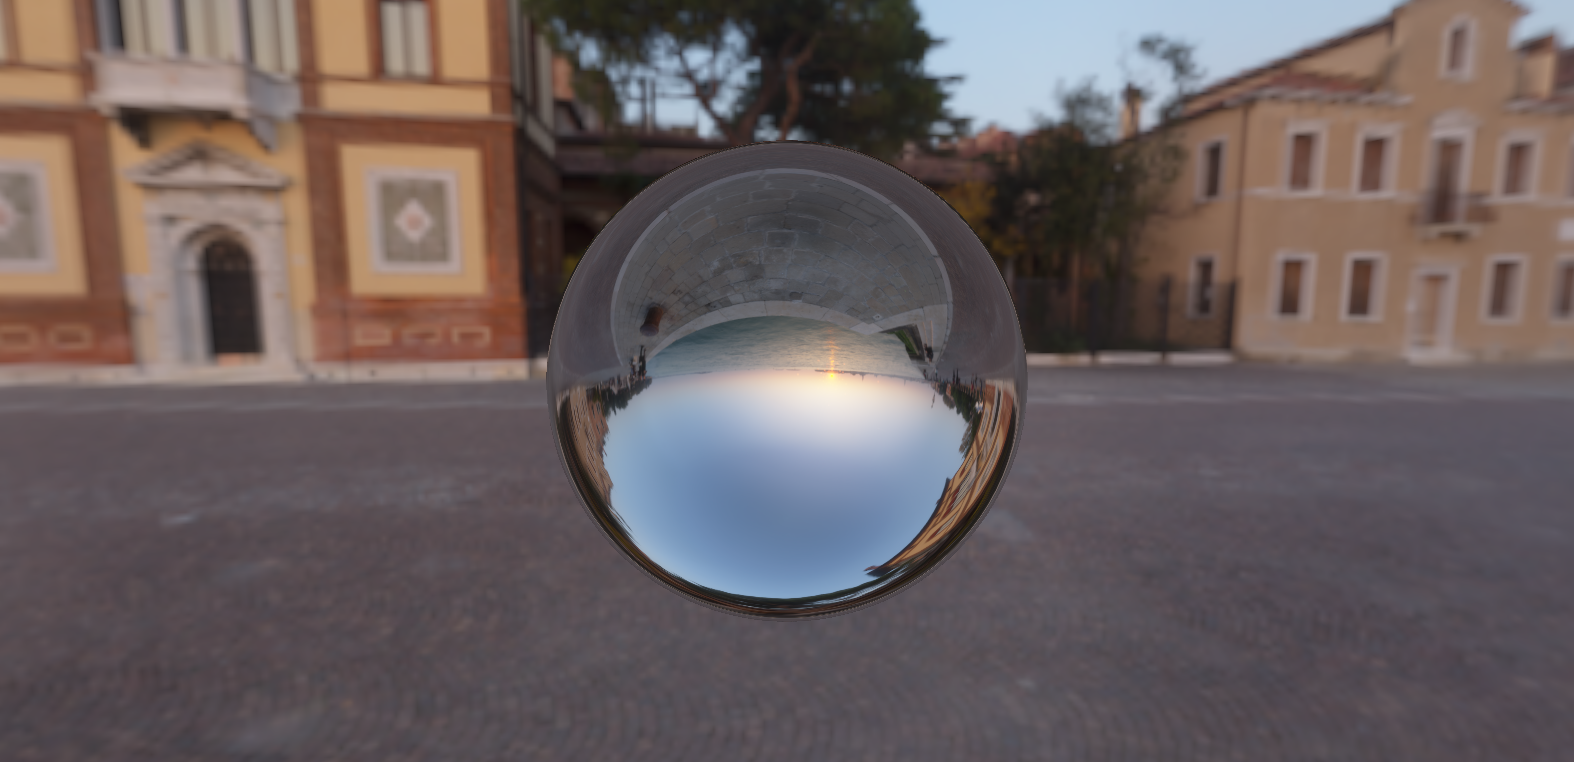
\includegraphics[width=\linewidth]{report-assets/final-renders/material-chrome-low-roughness.png}
    \caption{A chrome sphere with low roughness. The object reflects the HDR environment through the IBL specular path.}
    \label{fig:chrome}
\end{figure}

Figure~\ref{fig:roughness} shows the effect of roughness.
Low roughness uses sharp mip levels of the prefiltered cubemap.
High roughness uses blurrier mip levels and gives a softer reflection.

\begin{figure}[tb]
    \centering
    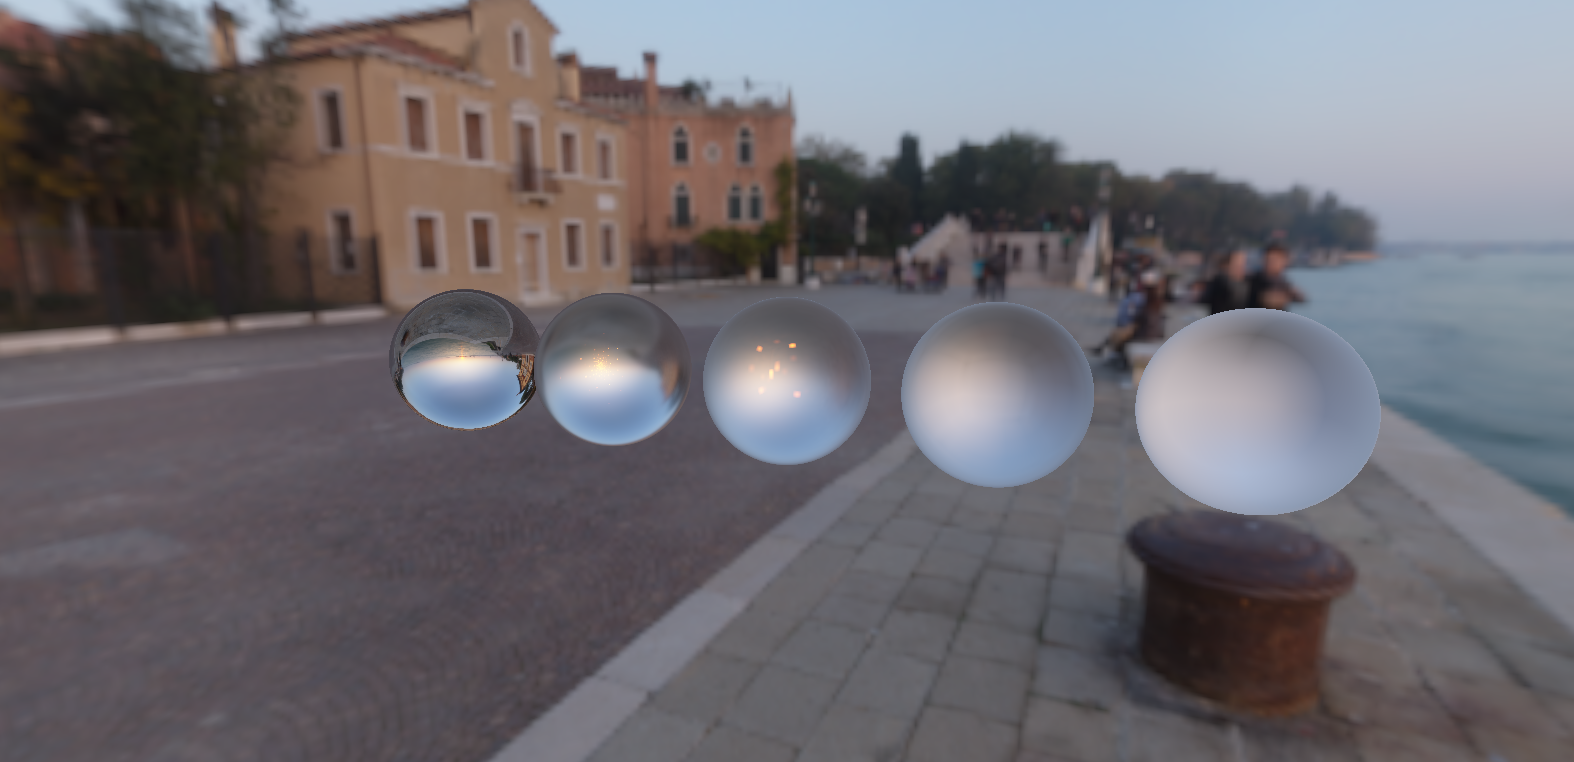
\includegraphics[width=\linewidth]{report-assets/04-roughness-strip.png}
    \caption{Roughness comparison from left to right: 0, 0.25, 0.5, 0.75, and 1.0.}
    \label{fig:roughness}
\end{figure}

Figure~\ref{fig:dragon} shows the Stanford Dragon lit by the same IBL shader as the sphere.
The model uses diffuse irradiance and specular IBL from the Venice Sunset environment.

\begin{figure}[tb]
    \centering
    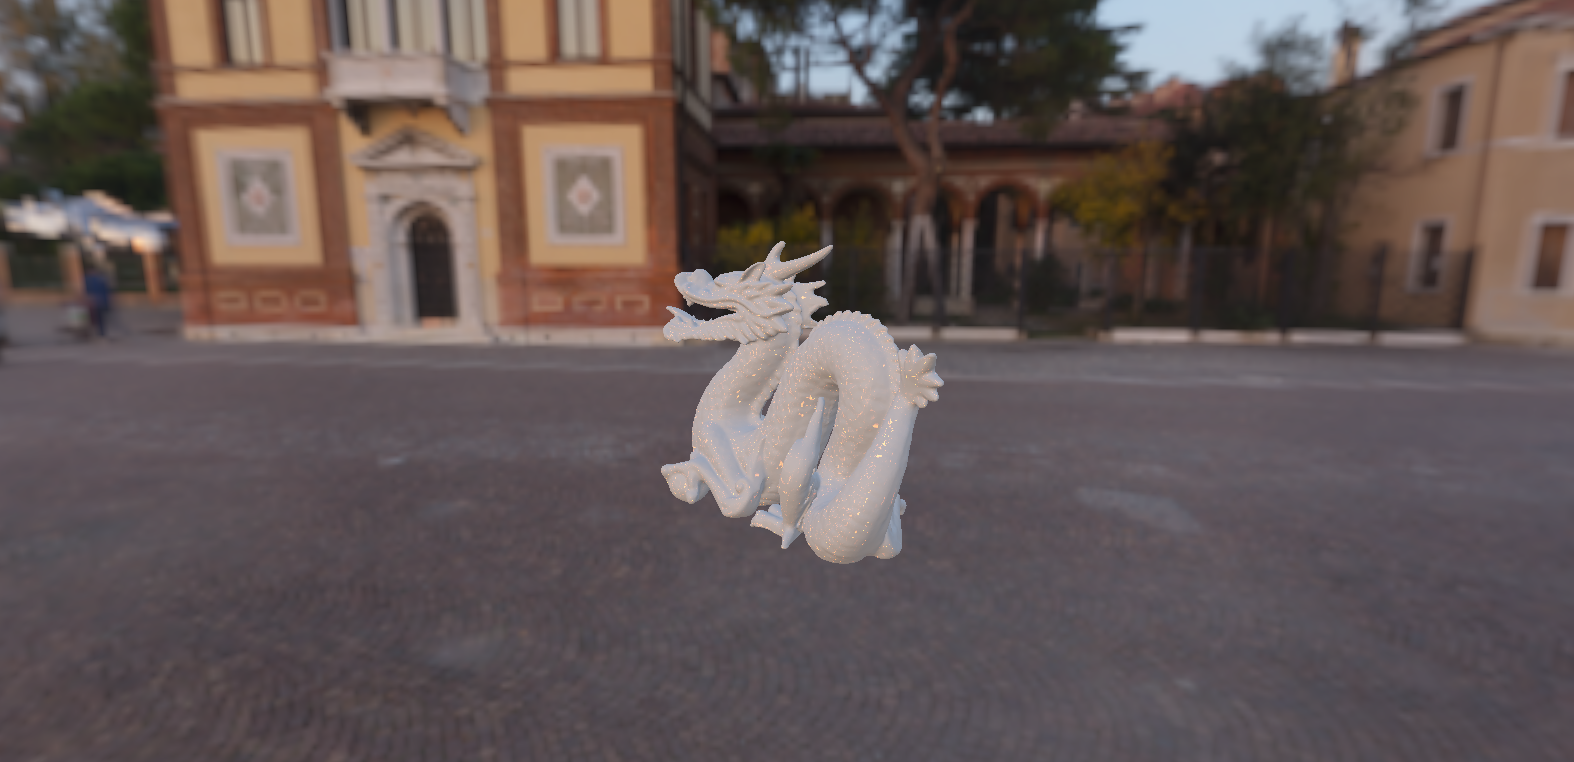
\includegraphics[width=\linewidth]{report-assets/final-renders/dragon-venice-plastic.png}
    \caption{The Stanford Dragon rendered with image-based lighting. The same shader is used for all meshes.}
    \label{fig:dragon}
\end{figure}

Figure~\ref{fig:environment} compares the same sphere under two HDR maps.

\begin{figure}[tb]
    \centering
    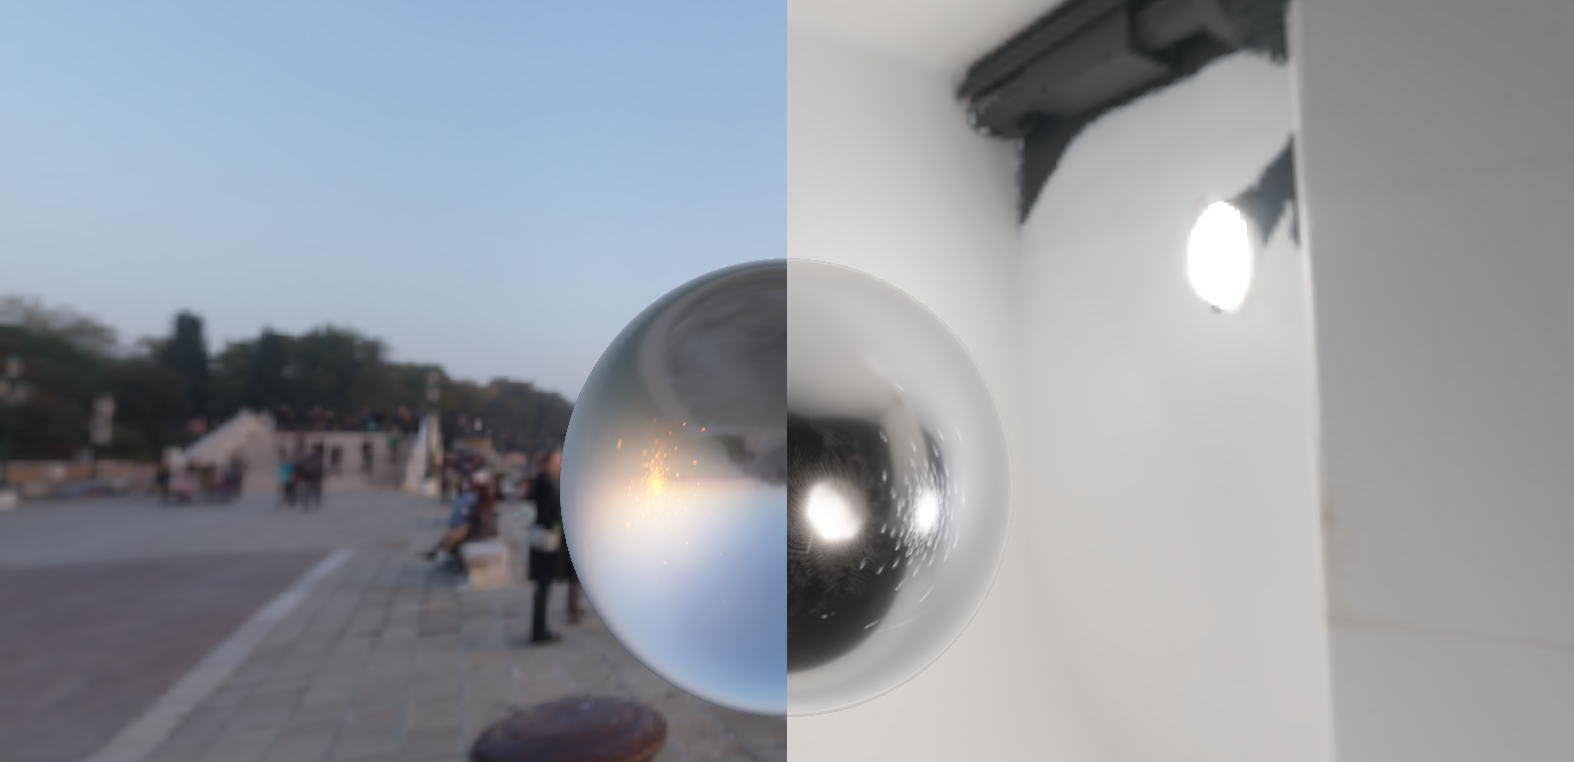
\includegraphics[width=\linewidth]{report-assets/08-environment-ab.png}
    \caption{Environment comparison with the same sphere, material, and camera. The left side uses Venice Sunset, while the right side uses Studio Small 09.}
    \label{fig:environment}
\end{figure}

Figure~\ref{fig:bunny} shows a diffuse Bunny under Kiara 1 Dawn.
The light comes from the irradiance cubemap, so the result is soft and low frequency.

\begin{figure}[tb]
    \centering
    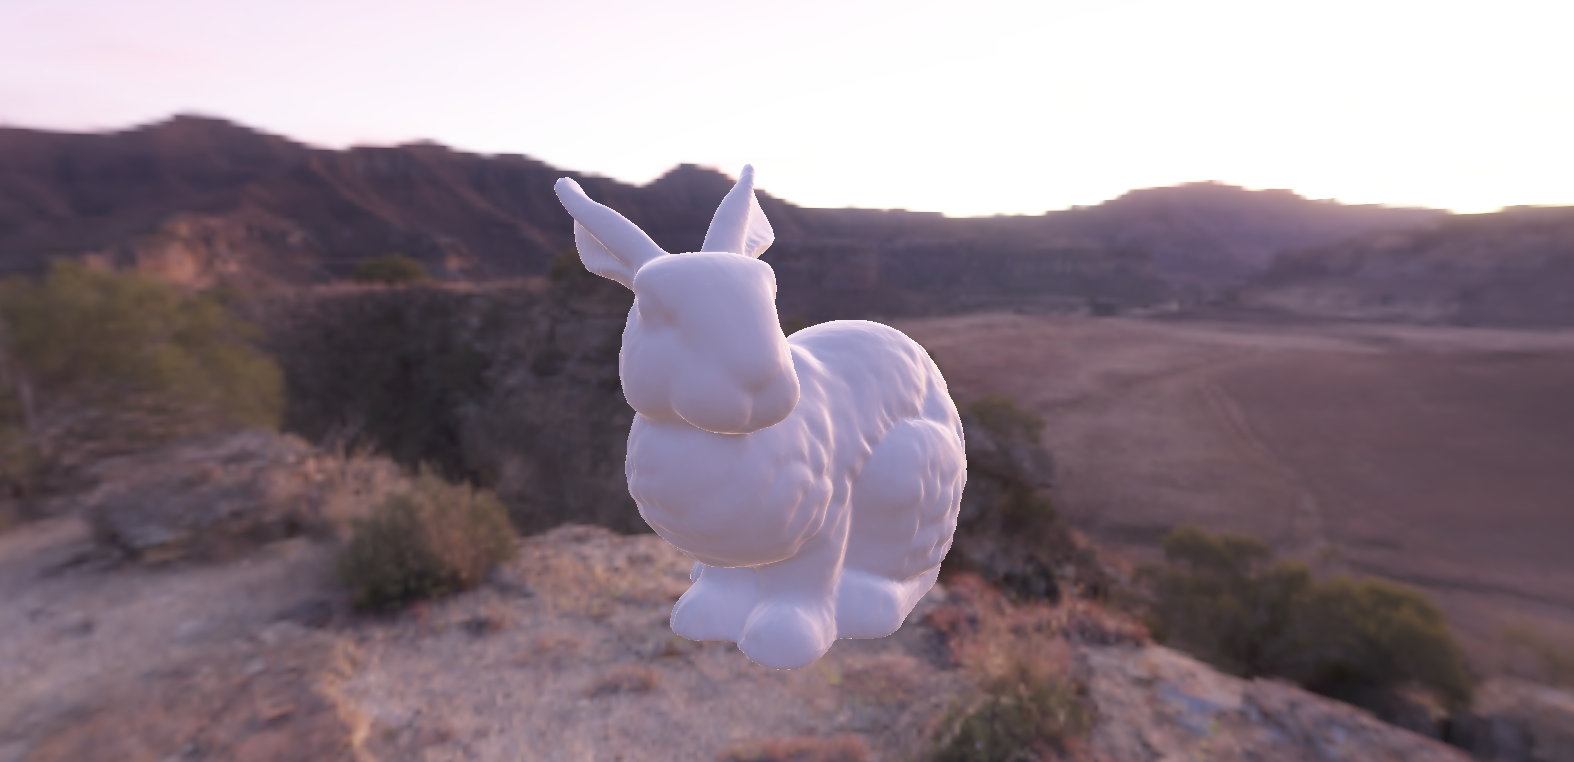
\includegraphics[width=\linewidth]{report-assets/final-renders/bunny-kiara-plastic.png}
    \caption{The Stanford Bunny under Kiara 1 Dawn. Diffuse irradiance gives soft environment lighting.}
    \label{fig:bunny}
\end{figure}

The screenshots show the main expected behavior.
Changing the environment changes the lighting and reflection.
Changing roughness changes the sharpness of the reflection.
Changing metallic changes the balance between diffuse and specular response.
The Stanford models use the same IBL path as the procedural sphere.

\section{Performance}

The app shows performance values in its stats panel.
Table~\ref{tab:renderperf} lists representative values measured on the test machine in Chrome/Edge with WebGPU.
The display was limited to about 60 FPS by the browser.

\begin{table}[tb]
    \centering
    \caption{Representative rendering performance from the stats panel.}
    \label{tab:renderperf}
    \resizebox{\linewidth}{!}{%
        \begin{tabular}{llllrr}
            \toprule
            Scene           & Model  & Vertices & Triangles & FPS & Frame time \\
            \midrule
            Studio Small 09 & Dragon & 437,645  & 871,414   & 60  & 16.7 ms    \\
            Venice Sunset   & Dragon & 437,645  & 871,414   & 60  & 16.7 ms    \\
            \bottomrule
        \end{tabular}
    }
\end{table}

Table~\ref{tab:preprocess} lists preprocessing times shown by the app for one Venice Sunset run.
These times depend on the GPU, browser, and driver.
The specular prefilter step is the most expensive step because it renders all cubemap faces for all mip levels.

\begin{table}[tb]
    \centering
    \caption{Representative preprocessing times for Venice Sunset.}
    \label{tab:preprocess}
    \begin{tabular}{llr}
        \toprule
        Step                       & Resolution               & Time   \\
        \midrule
        Equirectangular to cubemap & $512^2 \times 6$         & 91 ms  \\
        Irradiance convolution     & $64^2 \times 6$          & 101 ms \\
        Specular prefilter         & $256^2 \times 6$, 9 mips & 903 ms \\
        BRDF LUT                   & $256^2$                  & 101 ms \\
        \bottomrule
    \end{tabular}
\end{table}

All HDR IBL textures use \texttt{rgba16float}.
The prefilter pass uses 256 importance samples per face and mip level.
The BRDF LUT shader uses 1024 samples per pixel.

\section{Discussion and Limitations}

IBL moves much of the lighting work into preprocessing.
This makes the final render fast, since the shader mostly samples precomputed textures.
The quality depends on the HDR map, cubemap resolution, prefilter sample count, and mip levels.

The renderer is not a full global illumination renderer.
Objects do not cast contact shadows onto a ground plane.
They also do not affect the environment or bounce light onto each other.

Large Stanford models can take time to download and parse in the browser.
The Dragon works in this implementation, but its ASCII PLY file is much larger than the Bunny.
Binary mesh formats would load faster, but ASCII PLY keeps the loader simple for a seminar project.

\section{Conclusion}

This project implements a WebGPU image-based lighting renderer with HDR loading, equirectangular-to-cubemap conversion, diffuse irradiance, GGX specular prefiltering, a BRDF integration LUT, and PBR shading.
It renders a procedural sphere, the Stanford Bunny, and the Stanford Dragon with the same IBL pipeline.
The UI exposes material controls, environment switching, comparison views, and performance stats.
The results show real-time environment-based lighting and clear changes when the HDR map, metallic value, and roughness change.

\begin{thebibliography}{9}

    \bibitem{debevec2006ibl}
    P.~Debevec.
    \newblock Image-based lighting.
    \newblock In \emph{ACM SIGGRAPH 2006 Courses}, 2006.

    \bibitem{debevec1999ibml}
    P.~Debevec.
    \newblock Image-based modeling and lighting.
    \newblock \emph{ACM SIGGRAPH Computer Graphics}, 33(4):46--50, 1999.

    \bibitem{webgpu}
    W3C GPU for the Web Community Group.
    \newblock WebGPU and WebGPU Shading Language specifications.
    \newblock \url{https://www.w3.org/TR/webgpu/}, \url{https://www.w3.org/TR/WGSL/}.

    \bibitem{learnopengl}
    J.~de Vries.
    \newblock Physically Based Rendering and Image Based Lighting.
    \newblock LearnOpenGL.
    \newblock \url{https://learnopengl.com/PBR/IBL/Diffuse-irradiance}.

    \bibitem{polyhaven}
    Poly Haven.
    \newblock CC0 HDRI environments: Venice Sunset, Studio Small 09, and Kiara 1 Dawn.
    \newblock \url{https://polyhaven.com/}.

    \bibitem{stanfordscan}
    Stanford Computer Graphics Laboratory.
    \newblock The Stanford 3D Scanning Repository.
    \newblock \url{https://graphics.stanford.edu/data/3Dscanrep/}.

\end{thebibliography}

\end{document}
